
%(BEGIN_QUESTION)
% Copyright 2004, Tony R. Kuphaldt, released under the Creative Commons Attribution License (v 1.0)
% This means you may do almost anything with this work of mine, so long as you give me proper credit

Calculate all voltages, currents, and total power in this balanced Y-Y system:

$$\includegraphics[width=15.5cm]{i01994x01.eps}$$

\begin{itemize}
\item{} $V_{line} =$
\vskip 10pt
\item{} $I_{line} =$
\vskip 10pt
\item{} $V_{phase(source)} =$
\vskip 10pt
\item{} $I_{phase(source)} =$
\vskip 10pt
\item{} $V_{phase(load)} =$
\vskip 10pt
\item{} $I_{phase(load)} =$
\vskip 10pt
\item{} $P_{total} =$
\end{itemize}

\vskip 20pt \vbox{\hrule \hbox{\strut \vrule{} {\bf Suggestions for Socratic discussion} \vrule} \hrule}

\begin{itemize}
\item{} Identify which fundamental principles of electric circuits apply to each step of your analysis of this circuit.  In other words, be prepared to explain the reason(s) ``why'' for every step of your analysis, rather than merely describing those steps.
\item{} Suppose the center of the wye-connected load were connected to earth ground.  Determine the amount of voltage between each terminal of the wye-connected source and earth ground.
\end{itemize}

\underbar{file i01994}
%(END_QUESTION)





%(BEGIN_ANSWER)

\noindent
{\bf Partial answer:}

\medskip
%\item{} $V_{line} =$ 13.8 kV
%\item{} $I_{line} =$ 5.312 A
\item{} $V_{phase(source)} =$ 7.967 kV
\item{} $I_{phase(source)} =$ 5.312 A
\item{} $V_{phase(load)} =$ 7.967 kV
%\item{} $I_{phase(load)} =$ 5.312 A
\item{} $P_{total} =$ 126.96 kW
\end{itemize}

%(END_ANSWER)





%(BEGIN_NOTES)

\begin{itemize}
\item{} $V_{line} =$ 13.8 kV
\item{} $I_{line} =$ 5.312 A
\item{} $V_{phase(source)} =$ 13.8 kV / $\sqrt{3}$ = 7.967 kV
\item{} $I_{phase(source)} =$ 7.967 kV / 1500 $\Omega$ = 5.312 A
\item{} $V_{phase(load)} =$ 13.8 kV / $\sqrt{3}$ = 7.967 kV
\item{} $I_{phase(load)} =$ 7.967 kV / 1500 $\Omega$ = 5.312 A
\item{} $P_{total} =$ ($\sqrt{3}$) (13.8 kV) (5.312 A) = 126.96 kW
\end{itemize}

%INDEX% Electronics review: 3-phase electrical power 

%(END_NOTES)



